\documentclass[a4paper,10pt]{article}
\usepackage{hcolor}
\usepackage{color}
\usepackage{fancyhdr}
\usepackage[pdftex]{graphicx}

\def\RCS$#1: #2 ${\expandafter\def\csname RCS#1\endcsname{#2}}
\RCS$Date$
\RCS$Revision$


\setlength\topmargin{0in}
\setlength\headheight{0in}
\setlength\headsep{0.2in}
\setlength\textheight{24cm}
\setlength\textwidth{6.5in}
\setlength\oddsidemargin{0in}
\setlength\evensidemargin{0in}
\setlength\parindent{0.25in}
\setlength\parskip{0.25in}


\newcommand{\code}[1]{%
\begin{center}
  \fboxsep=10pt
  \fcolorbox{black}{green}
  {
       \parbox[c]{12cm}{
     \color{blue}{#1}}
  }
\end{center}}


% Title Page
\title{BankEfficiency documentation}
\author{Thomas Cokelaer}

\begin{document}
\bibliographystyle{unsrt}
\pagestyle{plain}
\fancypagestyle{plain}
\rfoot{}
\cfoot{\arabic{page} of \pageref{theend}}
\lfoot{}
\pagestyle{plain}
\lhead{BankEfficiency documentation -- v.\RCSRevision}



\maketitle
\section{Introduction}

BankEfficiency is a tool, which is available in lalapps/src/findchirp, that was primarely created to test efficiencies of template banks at detecting inspiralling compact binaries in the context of ground based detetectors. 

Although it relies heavily on LAL packages such as bank, inspiral and noisemodels packages, nevertheless it has its own sets of routines, which makes BankEfficiency a pretty long piece of code (about 4,000 lines) but also quite independant. BankEfficiency is quite modular, and the main core is pretty small (about 400 lines). It should therefore be easy to adapt it to your needs. 

\textbf{What BankEfficiency can do :}
\begin{itemize}
 \item Compute overlaps between a signal and a template bank
 \item Perform large Monte-Carlo simulations using condor and dag technology.
 \item Store results in XML format both for data mining and keep track of the parameters being used.
 \item Inject any type of signal that is available in LAL inspiral package
 \item Use any template bank that is available in LAL bank package
 \item Use any noise model that is available in LAL noisemodel package
\end{itemize}

\textbf{What BankEfficiency cannot do }
\begin{itemize}
 \item a multidetector anaylis
 \item analyse real noise, although implementation of an interface should be straigtforward.
 \item PTF filtering
 \item BCV spin filtering
\end{itemize}

BankEfficiency has become a powerful tool but it neccesiates a lot of input arguments, most of them having default values hardcoded. The documentation has two main objectives that are (1) explain what type of simulations you can performed with BankEfficiency, and (2) how to set the input parameters properly.

In the following we assume that the reader knows what is a template bank, what is matched filtering, what is a template, and what are the models such as EOB, PadeT1, TaylorT1 and so on. If not, you may look at one of the references in the bibliography 

\section{Tutorial}
In this section, I will introduce a few examples to show what type of simulations BankEfficiency and what is the ouput. 

\subsection{First example and outputs}
Let us start with a very simple example that has only two input parameters. This is possible because all parameters have default values. 

\code{lalapps\_BankEfficiency {-}{-}template EOB {-}{-}signal EOB}

Here, we specify both the signal and templates model to be based on EOB model. To do so, we use (\textbf{{-}{-}signal EOB}) and (\textbf{{-}{-}template EOB}). The code will inject an EOB signal and filter it through a template bank whose templates are also based on EOB signal. We'll come back on the template bank placement later on. Also, the components masses of the injected signal are randomised so that the total mass is uniformly distributed between 5 and 20 solar masses, which are the default values. The phase order of both the signal and templates are set to 2PN order by default. There are many other default values such as the sampling, the minimla match of the template bank\dots We'll see later how to change all these default values.

\textbf{Note that by defautl the initial phase of the signal is randomised but can be switch off using --no-start-pphase option}

The previous command returns a bunch of numbers on the screen. If not, most probably there was an error in the code.You may use the option \textbf{{-}{-}debug 33} to check any standard LAL errors. I would advide to always use this option

The next step is to understand what all these numbers are. From the output on the screen this is quite tedious. Luckily, at the end of the previous command, one can add an option to stored results in an XML file : \textbf{--xml-output} such as in the following example

 \code{lalapps\_BankEfficiency {-}{-}template EOB {-}{-}signal EOB {-}{-}debug 33 {-}{-}xml-output}

This option will create a file called \textbf{BankEfficiency-Result.xml} that contains (1) all the input parameters and (2) all the results of the simulation. The structure of the XML file is similar to all standard LIGO XML file.

Here, we assume that you are familiar with the \textbf{lwtprint} executables from ligotools. The output results of BankEfficiency are stored in XML format in a table that is called \textbf{bankefficiency} (no big caps). From now, you can extract the output of BankEfficiency using this kind of command: 

\code{lwtprint BankEfficiency-Result.xml -t bankefficiency -c mass1\_sim,mass2\_sim,snr}

where \textbf{-t bankefficiency } parses the bankefficiency outputs and \textbf{-c snr,mass1\_sim,mass2\_sim} means you want to extract the columns labelled \textbf{snr}, \textbf{mass1\_sim} and \textbf{mass2\_sim}. Of course, you need to know what are the column's name. At the end of this document (Sec.~\ref{default}), we provide the list of columns and their meaning 

In the previous example, we extracted the component masses as well as the SNR. Actually, this is the overlap between the signal and the template bank that is a single number for each injected signal. This single number is therefore a maximisation over time and parameter space of all the correlation/matched filtering performed during a simulation.

As you've probably noticed, the input parameters can be very succint. In this first example, we provide only 2 or 3 arguments. This simply means that many parameters are set by default. For instance the sampling is 2048Hz and  the template bank is based on a square placement and so on. In order to know all the default values, you can consult the header of BankEfficiency. A nicer way is again to look at the XML file. Indeed, all the parameters used for the simulation are stored in the \textbf{process\_params} table togethre with the version of the code that has been used, which is stored in \textbf{process} table. So, using the process\_params table you should be able to reproduce your results. 

Finally, if you use \textbf{BankEfficiency} as a standalone and add the option \textbf{--print-bank}, you will also have the template bank stored in a file called \textbf{BankEfficiency-Bank.xml}.

There are a few other possible outputs and we will come back to this later in this document.


\subsection{How to test a template bank}
BankEfficiency was design to test the efficiency of a template bank. To do so, you need to inject many signals at a time, and filter it through all the templates of the template bank. 

There are three important steps : 
\begin{enumerate}
 \item Set the signal model and its parameters
 \item Set the template and its parameters
 \item Set the template bank and its parameters
\end{enumerate}
The two last points seem similar (dealing with the template) but are completely independant. The template bank is a grid of points in the parameter space considered(e.g., component masses) and the templaete model can be anything. Ideally, the template bank should be constructed with the knowledge of template model. This is the case for the so-called SPA tempalte bank that is designed for TaylorF2 model. However, since other model such as TaylorT3, EOB are quite similar to the TaylorF2, you can use the same so-called SPA template bank for those models as well. 

Nothing prevent you to use this SPA template bank (the grid) with model based on something that can be very different such as Eccentric or amplitude corrected waveforms.

So, coming back to the template bank test, one really need to inject many signals to be able to quantify the efficiency of the template bank, that is the distribution of the overlaps in the parameter space. To do so, you can set the numner of simulations using  \textbf{--n 10000}. 

Then, to be realistic, the minimal match of the bank is set to \textbf{-- mm 95\%} (by default it is set to 80\%).

\code{lalapps\_BankEfficiency {-}{-}template EOB {-}{-}signal EOB  {-}{-}xml-output {-}{-}print-bank {-}{-}debug 33 {-}{-}n 10000 {-}{-}mm 0.95}

This command returns 10000 lines of numbers. So again, it is better to work with the XML file. BankEfficiency does not create any plots for you. So you can use whatever tool you prefer (matlab,xmgrace,...). However, within lalapps/src/findchirp package, there are 2 python files called plotbankefficiency.py (the executable) and inspiraltools.py (the library). Use the former one as follows : 

\code{python plotbankefficiency.py --glob 'BankEfficiency-Results.xml' --verbose --user-tag 'test'} so as to generate a bunch of plots you may found useful. For instance, Fig.\ref{fig:snr1} shows the distribution of the overlaps versus total mass.

\begin{figure}
\centering
 %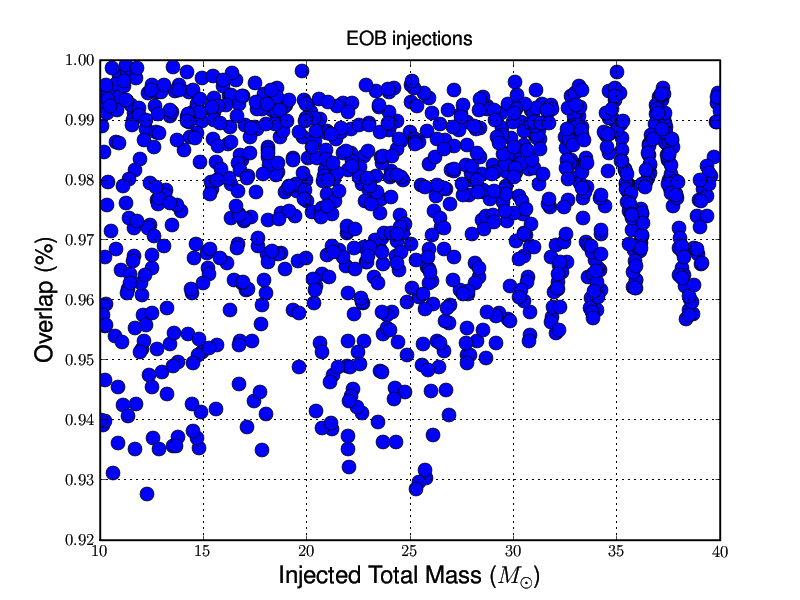
\includegraphics[width=0.4\textwidth]{bankefficiencydoc_snr_versus_totalmass.png}
\caption{\label{fig:snr1} Overlaps versus total mass}
\end{figure} 

Note that the XML table does not contains all the physical information you may want. It is quite light though because only 2 mass parameters are stored for the injection and for the btemplate that gives the best SNR. Indeed, other set of parameters can be computed a posteriori.

\subsection{Noise and Signal}\label{model}
In the two previous examples, we consider noiseless simulations. BankEfficiency was indeed created to check the overlap betweem a template bank and an injection. But, thanks to the noisemodel package, it is straightforward to use simulation where the signal is buried in some noise (you can even set the signal amplitude to be null so as to study only the noise).  This can be done as follows : 
\code{lalapps\_BankEfficiency {-}{-}template EOB {-}{-}signal EOB {-}{-}debug 33  {-}{-}mm 0.95 {-}{-}n 10000  {-}{-}xml-output {-}{-}print-bank  {-}{-}simulation-type NoiseAndSignal {-}{-}signal-amplitude 25}

The noise is a colored gaussian noise with a variance such that the average SNR is set by \textbf{{-}{-}signal-amplitude} to 25. 

This is very useful to perform test of the Fisher matrix by testing the dispersion/accuracy of the mass parameters. 

Usually, you would want the mass of the injection to be fixed instead  of being randomized. This can be done by fixing the individual masses as follows: 
\code{lalapps\_BankEfficiency {-}{-}template EOB {-}{-}signal EOB {-}{-}mm 0.95 {-}{-}n 10000  {-}{-}xml-output {-}{-}print-bank  {-}{-}simulation-type NoiseAndSignal {-}{-}signal-amplitude 25 {-}{-}m1 10 {-}{-}m2 10}

Another option related to the noise is that you may want to specify different type of colored noise, which currently are LIGOI, LIGOA, VIRGO, EGO, TAMA for initial LIGO, advanced LIGO, VIRGO, Einstein Telescope and TAMA, which can be fixed by \textbf{{-}{-}noise-model}.


\code{lalapps\_BankEfficiency {-}{-}template EOB {-}{-}signal EOB {-}{-}mm 0.95 {-}{-}n 10000  {-}{-}xml-output {-}{-}print-bank  {-}{-}simulation-type NoiseAndSignal {-}{-}signal-amplitude 25 {-}{-}m1 10 {-}{-}m2 10 {-}{-}noise-model LIGOA}

using the --print-psd option, the PSD will be saved in \textbf{BankEfficiency-PSD.dat}.

\subsection{template bank related}\label{bank}
Let us now look in more details at the parameters related to the template bank itself.

First of all, there are only two specific type of template bank available at the moment that are in the LAL bank package. The first template bank is the SPA template bank for physical modesl such as EOB,TAylor,Pade. The second one is a BCV template bank that is being called if \textbf{{-}{-}template} is set to \textbf{BCV}, which is discussed later on. Let us focus on the SPA template bank for now. 

There are two types of placement : square and hexagonal. Historically, square placement was implemented and can be called using \textbf{{-}{-}bank-grid-spacing SquareNotOriented}. Then hexagonal placement was imlemented and can be called using \textbf{{-}{-}bank-grid-spacing Hexagonal}

\textbf{Technical:}
A template bank is constructed using the metric components of the signal/template manifold. The metric components are computed by calculating quantities such as the  moments, whihc in turn are integrals from a lower cut-off frtequency to an upper cutoff frequency. The latter is  by default set to Nyquist frequency. One can force this upper cut-off frequency to be a fixed value by setting \textbf{{-}{-}bank-ffinal}. One can also recompute the moments for each template so that the upper cutoff frequency is the last stable orbit. This option is not et fully implemented but can be set on using \textbf{{-}{-}compute-moments} to recompoute the Gammas appropriately. 

By default the minimal match of the template bank is 80\% but you can change it using \textbf{{-}{-}mm} option.

To set the masse range to which the bank is efficient, use \textbf{{-}{-}bank-mass-range 1 3}.

There is also the possibility to create a template bank that has a fine grid. The fine grid is implemented within bankEfficiency and requires this parametres: 
\begin{itemize}
 \item \textbf{{-}{-}t0-fine-range} 2 values to set the t0 range
\item \textbf{{-}{-}t3-fine-range} 2 values to set the tau3 range
\item \textbf{{-}{-}t0-fine-bin} number of bins in this dimension
\item \textbf{{-}{-}t3-fine-bin} number of bins in this dimension
\end{itemize}



\subsection{Eccentricity related}\label{eccentricity}
If the signal is set to \textbf{Eccentricity} (using the {-}{-}signal option), then you can set the eccentricity of the simulated signals by using a range. The eccentricity will be uniformly distributed witin the two values that define this range. For instance :
\code{lalapps\_BankEfficiency {-}{-}template TaylorT3 {-}{-}signal Eccentricity {-}{-}mm 0.95 {-}{-}n 10000  {-}{-}xml-output --signal-eccentricity-range 0 0.4}

Note that the Eccentric model is only implemented at the Newtonian order for the moment. Therefore, one must specify the Newtonian order on the command line argument (by default the 2PN is used). If not, the code will fail. 

So, stricly speaking, the command above should have been : 
\code{lalapps\_BankEfficiency {-}{-}template TaylorT3 {-}{-}signal Eccentricity {-}{-}mm 0.95 {-}{-}n 10000  {-}{-}xml-output --signal-eccentricity-range 0 0.4 --signal-order 0}

where the number 0 stands for Newtonian.

There is no eccentric template bank. However, one can set the template bank to be based on SPA bank (optimised for a search that uses 2PN template) but place a eccentric template on each point of the grid. Yet, by default all template will have their eccentricity fixed to zero. So, really, this is not an eccentric template bank. To do so, one would need the metric in the eccentric dimension and create a template bank adequately. Yet, there is a naive template bank that is called by using the option \textbf{{}{}bank-eccentricity-range} followed by  a range of values and a number of bins. The template will be nbins times the original template bank each of them having a different value of eccentricity. This is naive because it assumes that the metric is flat in the eccentric dimension even though this is clearly not the case. However, one can already test how we can recover eccentric waveforms and performed some tests. 

\code{lalapps\_BankEfficiency {-}{-}template TaylorT3 {-}{-}signal Eccentricity {-}{-}mm 0.95 {-}{-}n 10000  {-}{-}xml-output --signal-eccentricity-range 0 0.4 --signal-order 0 --bank-eccentric-range 0 0.4 --bank-eccentricity-bins 10}

\subsection{BCV related functions}\label{bcv}
In this section, we show how to test a template bank based on BCV template and how a BCV template bank can detect signals based on other models such as EOB. 

First, the BCV template bank itself is set up using this arguments : 
--bank-alpha 0.01
--bank-psi0-range 10 250000
--bank-psi3-range -2200 -10
--bank-fcut 2 6
--bank-number-fcuts
--bank-inside-polygon

The BCV signal can be injected. We can force the psi0/psi values using --psi0 and -psi3 options. 
otherwise the --signal-psi0-range and --signal-psi3-range  need to be fixed or default values will be used instead.

Concerning the filtering there is an option to avoid the alpha constraint to be used --no-alpha-constraint --alpha-constraint



\subsection{Amplitude Corrected related}\label{ampcor}
To use the maplitude corrected waveforms, one can simply set the AmpCorPPN in --signal and --template. The order needs alos to be set by using --signal-amp-order  and --template-map-order

Concerning the input parameter of the signal, one also need to set the range of inclination and polarisation.  --signal-inclination-rane --signal-polarisation-range
Note however that because the signal are normalised with resepcte to their energy, the effect of the inclination on the amplitude of the signal wont be seen.

The template bank is based on SPA placement.

The filtering is the standard filtering in quadrature. 

\subsection{others}\label{others}
There are a few other options. Some of whihc can be useful.
\subsubsection{force the length of the signal}
In principle BankEfficiency estimates the longest length of all templates and all possible signals and allocate memory such that the vectors are long enough. If you still want to increase the size you can either use \textbf{{-}{-}num-seconds} to fix the size yourself (but you need to know the optimal length) or multiply the standard values by a factor using \textbf{{-}{-}}.
\subsubsection{lower cut off}
--fl --fl-template  are equivalent and fix both the fl of the template and fl of the integration.

--fl-signal
\subsubsection{fast option}
There is a fast option to perform the simulation that can be very powerful. It is based on the metric of the signal. So if the template and the signal are based on the same approximant, it can be used very safely. It is switch on by using \textbf{{-}{-}fast-simulation} and \textbf{{-}{-}e-match}, which is set to 0.5. Briefly, the match is unity when the signal and template are identical. As soon as they differ, the match decrease. Having a match of 0.5 means that the loss of SNR is 50\%. Since it is not normalised, it can take negative values.


\subsubsection{BHNS injection}
There are many ways to choose the parameters of the signal to be injected. By default, the total mass is uniformly distributed and the component masses are set using the option \textbf{{-}{-}signal-mass-range}. You can overwrite this option by using together the \textbf{{-}{-}m1} and \textbf{{-}{-}m2} options to force the component masses to be fixed. Similarly, if you prefer to work with the chirp times parameters, you can use 
\textbf{{-}{-}tau3} and \textbf{{-}{-}tau0}. Finally, there is an option to force the masses to be such that the binary system is a BHNS system, that is the first component mass in in the range [1,3] and the second component mass is larger than 3. This option is \textbf{{-}{-}bhns-injection}. Of course you need to be sure that \textbf{{-}{-}signal-mass-range} has a range that include the value 3.

\subsubsection{check the code}
--check/faithfulness and --no-start-phase
--print-snr-histo

when --check is used, some parameters are not overwritten : flower, order, approximant,eccenticity,fFinal. only the mass parameetres. 
\section{Deploy your DAGs and CONDOR jobs}\label{dagandini}
\subsection{ini file}\label{ini}
\begin{verbatim}
[main]
executable=./lalapps_BankEfficiency

[general]
mm=0.95
sampling=2048
fl=40

[bank]
bank-grid-spacing=Hexagonal

[signal]
signal=EOB

[simulation]
ntrial=1000
njobs=100
\end{verbatim}

fix your ini file so that it does what you want.

\subsection{Generate the sub abd dag files.}\label{dag}
\code{python bep.py --config-file bep.ini}

\code{condor\_submit\_dag -maxjobs 100  -f bep.dag}


\section{Meaning of the bankefficiency XML table}\label{xml}
\begin{description}
\item[psi0] The first BCV parameter of the template
\item[psi3] The second BCV parameter of the template
\item[psi0\_sim] The first BCV parameter of the injection
\item[psi3\_sim] The second BCV parameter of the injection
\item[tau0] The first mass parameter of the template
\item[tau3] The second mass parameter of the template
\item[tau0\_sim] The first mass parameter of the injection
\item[tau3\_sim] The second mass parameter of the injection
\item[ecc] eccentricity of the best templates
\item[ecc\_sim] eccentricity of the signal
\item[ffinal] ffinal of the best templates
\item[ffinal\_sim] ffinal of the injection
\item[mass1\_sim] The first mass parameter of the injection
\item[mass2\_sim] The first mass parameter of the injection
\item[phase\_sim] The initial phase of the injection
\item[snr] the best overlap maximised over all template bank and time
\item[snr\_at\_ta] irrelevant for now
\item[phase] the phase of the best template
\item[alpha\_f] the alpha\_f value of the best template (BCV related)
\item[time] the time of arrival of the best template
\item[time\_sim] 
\item[nfast] number of templates really used
\end{description}

\section{Arguments and their default values}\label{default}
--bank-alpha 0.01\\
--bank-fcut-range\\
--bank-ffinal\\
--bank-inside-polygon\\
--bank-grid-spacing\\
--bank-number-fcut\\
--bank-mass-range 5 20\\
--bank-max-total-mass\\
--bank-min-total-mass\\
--bank-psi0-range 10 250000\\
--bank-psi3-range -2200 -10\\
--debug\\
--bank-eccentricity-range \\
--bank-eccentricity-bins\\ 
--e-match 0.5\\
--template-fl 40\\
--fl 40\\
--h\\
--ascii2xml\\
--m1\\
--m2\\
--mm 0.80\\
--ntrial 1\\
--noise-amplitude \\
--noise-model\\
--num-seconds\\
--psi0\\
--psi3\\
--sampling 2048\\
--seed\\
--signal EOB\\
--signal-alpha\\
--signal-amp-order\\
--signal-alpha1\\
--signal-alpha2\\
--signal-amplitude\\
--signal-eccentricity-range\\
--signal-ffinal\\
--signal-fl 40\\
--signal-inclination-range\\
--signal-polarisation-range\\
--signal-mass-range\\
--signal-tau0-range\\
--signal-tau3-range\\
--signal-order\\
--signal-nstartpad\\
--signal-psi0-range\\
--signal-psi3-range\\
--signal-random-nstartpad\\
--signal-max-total-mass\\
--signal-min-total-mass\\
--simulation-type\\
--t0-fine-range\\
--t3-fine-range\\
--t0-fine-bin\\
--t3-fine-bin\\
--no-start-phase\\
--tau0\\
--tau3\\
--template EOB\\
--template-order\\
--template-amp-order\\
--user-tag\\
--ambiguity\\
--alpha-constraint\\
--bhns-injection\\
--no-alpha-constraint\\
--print-best-overlap\\
--faithfulness\\
--check\\
--print-psd\\
--print-snr-histo\\
--verbose\\
--version\\
--print-bank\\
--compute-moments\\
--xml-output\\
--print-prototype\\
--fast-simulation\\

\section{FAQs}\label{faqs}
\subsection{Why BankEfficiency fails without any error message? }
Usually, the code is quite robust but there are a few places where it may fail. One is related to the size of the vectors not being long enough. By default we optimize the memory allocation by fixing the vector length to a minimal value. This value is estimated as twice the length of the longest template/signal to be used. If this estimation length is not done properly, when a signal is generated and overtakes this length, the program will fail.

An other reason could be related to the PN order not being set properly.

Usually, with a segmentation fault, this is related to vecrtor not being set properly.


% bibliography : bank papers : square, hexa, bcvspin, S3SBBH, reinhard, owen, Sathya,
\begin{thebibliography}{99}
\bibitem{LIGO}
A. Abramovici {\it et al.}, Science {\bf 256}, 325 (1992);
B. Abbott, {\it et al.}, Nuclear Inst. and Methods in Physics 
Research, A {\bf 517/1-3} 154 (2004).

\bibitem{VIRGO}
B. Caron {\it et al.}, Class. Quantum Grav. {\bf 14}, 1461 (1997);
F. Acernese {\it et al.}, {\em The Virgo detector,} 
Prepared for 17th Conference on High Energy Physics (IFAE 2005) (In Italian), 
Catania, Italy, 30 Mar-2 Apr 2005,  AIP Conf. Proc. {\bf 794}, 307-310 (2005).

\bibitem{damir}
F.~Beauville et al, Class.\ Quant.\ Grav.\ \textbf{22}, 4285, (2005).

\bibitem{Owen96}B.~Owen, Phys.\ Rev.\  D\textbf {53}, 6749 (1996).

\bibitem{OwenSathyaprakash98} B.~Owen, B.~S.~Sathyaprakash 1998 Phys.\ Rev.\ 
D \textbf{60} 022002 (1998).

\bibitem{squarebank}
S.~Babak and R.~Balasubramanian and D.~Churches and T.~Cokelaer and B.~S.~Sathyaprakash 2006 \textit{Class.\ Quantum Grav.\ }
\textbf{23} 5477

\bibitem{hexabank} T.~Cokelaer 2007 \textit{Gravitational Wave Detections of Inspiralling Compact Binaries: Hexagonal Template Placement and Physical Template Families}, (\textit{Preprint} gr-qc/0706.4437v1), Phys. Review D 76, 10, 2007 (15 Nov 2007) 


\bibitem{bcvbank} T.Cokelaer, 2007, \textit{A template bank to search for gravitational waves from inspiralling compact binaries: II. Phenomenological model}
Class. Quantum Grav. 24 (2007) 6227-6242 


\bibitem{BDI95} L. Blanchet, T. Damour and B.R. Iyer, Phys.\ Rev.\ D {\bf 51},5360 (1995).

\bibitem{LAL} LSC Algorithm Library LAL,\\
{\tt http://www.lsc-group.phys.uwm.edu/daswg/\-projects/lal.html}

\bibitem{LIGOS3S4}
B.~Abbott {\it et al.}, LIGO Scientific Collaboration, gr-qc/0704.3368v2,
(2007)

\bibitem{PSDs}
T.~Damour and B.R.~Iyer and B.S.~Sathyaprakash, Phys.\ Rev.\ D
\textbf{63}, 044023 (2001).

\end{thebibliography}


\label{theend}

\end{document}          

